\documentclass{article}

\usepackage[a4paper, margin=2cm]{geometry}
\usepackage[utf8]{inputenc}
\usepackage[T1]{fontenc}

\usepackage[czech]{babel}
\usepackage{fvextra}
\usepackage{csquotes}
\usepackage{parskip}

\usepackage{float}
\usepackage{amsmath}
\usepackage{siunitx}
\usepackage[shortlabels]{enumitem}
\usepackage{graphicx}

\usepackage[hidelinks, unicode, pdfusetitle]{hyperref}

\title{35-3-X1 Obvody}
\author{Benjamin Swart}

\graphicspath{{./images/}}

\begin{document}
\maketitle

\section{Plán}

Algoritmus bude fungovat zhruba takto:

Postupně budeme potřebným volným místům přidělovat rezistor. Pro každé místo se pokusíme najít buď volný rezistor, nebo sekvenci posunů již použitých rezistorů, která zaplní nově přidané místo a jednomu ze starých míst přidělí nový nepoužitý rezistor.

Dejme tomu, že máme například tato místa s množinami platných rezistorů $R$ a přiřazenými rezistory $r$:

\begin{enumerate}[a)]
    \item $R_a = \left[1 \unit{\ohm}; 5 \unit{\ohm}\right]; r_a = 5 \unit{\ohm}$
    \item $R_b = \left[5 \unit{\ohm}; 6 \unit{\ohm}\right]; r_b = 6 \unit{\ohm}$
    \item $R_c = \left[6 \unit{\ohm}; 7 \unit{\ohm}\right]; r_c = 7 \unit{\ohm}$
    \item $R_d = \left[7 \unit{\ohm}; 9 \unit{\ohm}\right]; r_d = 8 \unit{\ohm}$
    \item $R_e = \left[9 \unit{\ohm}; 9 \unit{\ohm}\right]; r_e = 9 \unit{\ohm}$
\end{enumerate}

Chceme do obvodu přidat místo s $R = \left[8 \unit{\ohm}; 9 \unit{\ohm}\right]$. Jedním řešením je přidělit novému místu $r = 8 \unit{\ohm}$, a změnit $r_d = 7 \unit{\ohm}$, $r_c = 6 \unit{\ohm}$, $r_b = 5 \unit{\ohm}$ a $r_a = 4 \unit{\ohm}$.

Dá se říci, že pokud přidáváme místo s množinou hodnot rezistorů $R$, tak můžeme množinu $R$ rozšířit o sjednocením všech množin hodnot míst, kterým byly přiděleny rezistory s hodnotou v $R$, a to rekurzivně.

\section{Implementace}

Zbývá jen vymyslet, jak tyto sekvence přesunů hledat.

Budeme si udržovat seřazenou množinu, například červeno-černý strom, všech aktuálně přiřazených rezistorů. Pokaždé, když začneme přidávat nové místo, tak si vytvoříme kopii této množiny. Projdeme všechny platné intervaly pro toto místo a najdeme v nich všechny přiřazené rezistory. Tato přiřazení odstraníme s z naší kopie množiny a uložíme si je do fronty. Přiřazení z fronty zpracujeme stejným způsobem a provedeme tedy vyhledávání do šířky. Postupně si takto vybudujeme seznam všech míst dosažitelných přesuny rezistorů. Pro každý dosažitelný rezistor si také zapamatujeme, skrz který předchozí rezistor je dosažitelný.

Množina $R$, která představuje všechny hodnot rezistorů, jejichž přiřazením můžeme problém nějakou sekvencí přesunů vyřešit, bude sjednocení všech intervalů platných hodnot nalezených dosažitelných míst.

Dejme tomu, že máme přiřazené rezistory R1 až R6 takto:

\begin{center}
    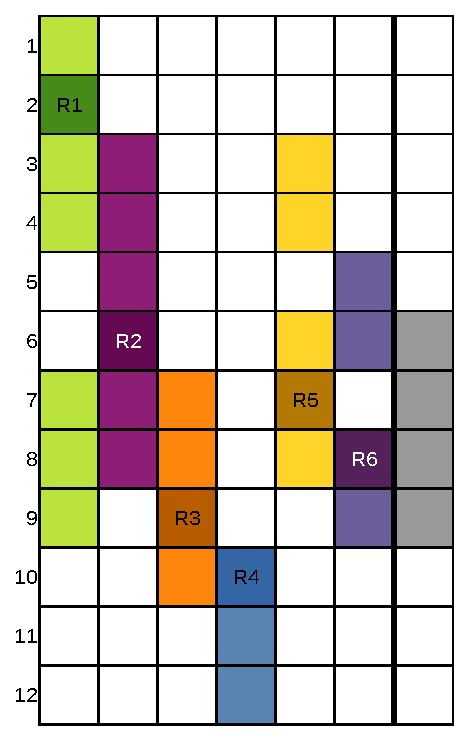
\includegraphics{intervals.pdf}
\end{center}

Barevná políčka označují intervaly platných odporů pro existující místa, tmavá políčka označují aktuálně přiřazený rezistor. Přidáváme místo s intervalem označeným šedě. Dosažitelné jsou všechny rezistory až na R1. Rezistor R4 je dosažitelný skrz R3, ostatní přímo. Množina $R$ bude $\left[3 \unit{\ohm}; 12 \unit{\ohm}\right]$. Jedno z platných řešení by tedy bylo přidělit místu R4 rezistor o hodnotě 11 \unit{\ohm}, nové uvolněný rezistor s odporem 10 \unit{\ohm} přiřadit R3 a novému rezistoru přidělit nově uvolněnou hodnotu 9 \unit{\ohm}. Jiné řešení by bylo přidělit R2 rezistor s hodnotou 4 \unit{\ohm} a novému místu přidělit hodnotu 6 \unit{\ohm}.

Nyní nám zbývá jen najít nějaký vhodný rezistor, jehož přidáním spustíme sekvenci přesunů. Množinu $R$ získáme snadno pomocí seřazeného seznamu začátků a konců intervalů dosažitelných rezistorů. Projdeme všechny prvky této množiny a zkontrolujeme, jestli je tato hodnota volná. Pokud volná je, tak najdeme jeden rezistor, v intervalu kterého se tato hodnota nachází, a přiřadíme mu tuto novou hodnotu. Jeho starou hodnotu přiřadíme rezistoru, skrz který jsme ho při prohledávání našli, a takto pokračujeme, dokud nepřiřadíme uvolněnou hodnotu přidávanému rezistoru.

\section{Analýza složitosti}

Tento algoritmus postupně projde všech $n$ míst.

Prohledávání do šířky za účelem nalezení dosažitelných rezistorů navštíví nejvýše $k$ intervalů, pro každý z nichž provede operaci na červeno-černém stromě. Prohledávání tedy zabere $\mathcal{O}(k \log n)$ času. Nalezení průniku intervalů zabere $\mathcal{O}(k \log k)$ času. Jelikož s procházením prvků množiny $R$ přestaneme jakmile najdeme volné místo, tak vyhledávání zabere nejvýše $\mathcal{O}(n)$ času, protože nemůžeme najít více jak $n$ zabraných hodnot rezistorů. V $\mathcal{O}(k)$ najdeme místo, kterému můžeme nalezenou hodnotu přiřadit a v $\mathcal{O}(n \log n)$ zvládneme také provést nalezenou sekvenci přesunů. (Musíme pracovat s červeno-černým stromem.)

Jedno přidání místa jsme tedy schopni zpracovat v $\mathcal{O}(k \log k)$. Celý algoritmus poběží v čase $\mathcal{O}(nk \log k)$ a bude potřebovat $\mathcal{O}(n + k)$ paměti.

\end{document}
